\newpage
\section{Plan de Implantación y Pruebas}
\label{cap:plan_implantacion}

\lstdefinelanguage{YAML}{
  keywords={true,false,null,y,n},
  keywordstyle=\color{blue}\bfseries,
  basicstyle=\ttfamily\footnotesize,
  rulecolor=\color{black},
  aboveskip={1.5\baselineskip},
  columns=fixed,
  showstringspaces=false,
  extendedchars=true,
  breaklines=true,
  backgroundcolor=\color{gray!5},
  frame=single,
  identifierstyle=\color{black},
  stringstyle=\color{orange}\ttfamily,
  commentstyle=\color{teal}\ttfamily,
  sensitive=false,
  comment=[l]{\#},
  morestring=[b]',
  morestring=[b]"
}

La materialización de la arquitectura teórica propuesta exige una metodología rigurosa para el ensamblaje físico, la configuración del \textit{software} perimetral y la validación empírica de todos los subsistemas. En este capítulo se detallan las fases de despliegue del prototipo, el esquema de conexionado físico y de pines de los nodos de instrumentación, y el protocolo de pruebas diseñado para certificar el cumplimiento de los requisitos funcionales, así como la tolerancia a fallos del motor lógico local.

\subsection{Fases del despliegue del sistema}
\label{sec:despliegue}
La implantación de la infraestructura domótica local se ejecutó siguiendo un modelo iterativo e incremental, estructurado en las siguientes fases secuenciales:
\begin{enumerate}
    \item \textbf{Aprovisionamiento y validación analógica:} ensamblaje preliminar de los componentes electrónicos en placa de pruebas (\textit{breadboard}) para la medición de caídas de tensión mediante multímetro, la calibración física de umbrales mediante el potenciómetro de precisión integrado en el módulo de detección acústica y la verificación general del comportamiento eléctrico en frío, minimizando el riesgo de cortocircuitos.
    \item \textbf{Despliegue del núcleo lógico perimetral:} instalación del sistema operativo subyacente (Raspberry Pi OS) en el servidor perimetral (Raspberry Pi 4 con 1\,GB de RAM) y el despliegue del servidor central Home Assistant Container y la suite ESPHome como contenedores independientes aislados en Docker. En esta fase se configuró el motor de base de datos local SQLite y su base de datos (\texttt{home-assistant\_v2.db}), definiendo las políticas de depuración y retención del historial para garantizar el rendimiento en un hardware con limitaciones de memoria y almacenamiento. El estado operativo de los contenedores desplegados se muestra en la Figura~\ref{fig:portainer_containers}.
    
    \begin{figure}[H]
        \centering
        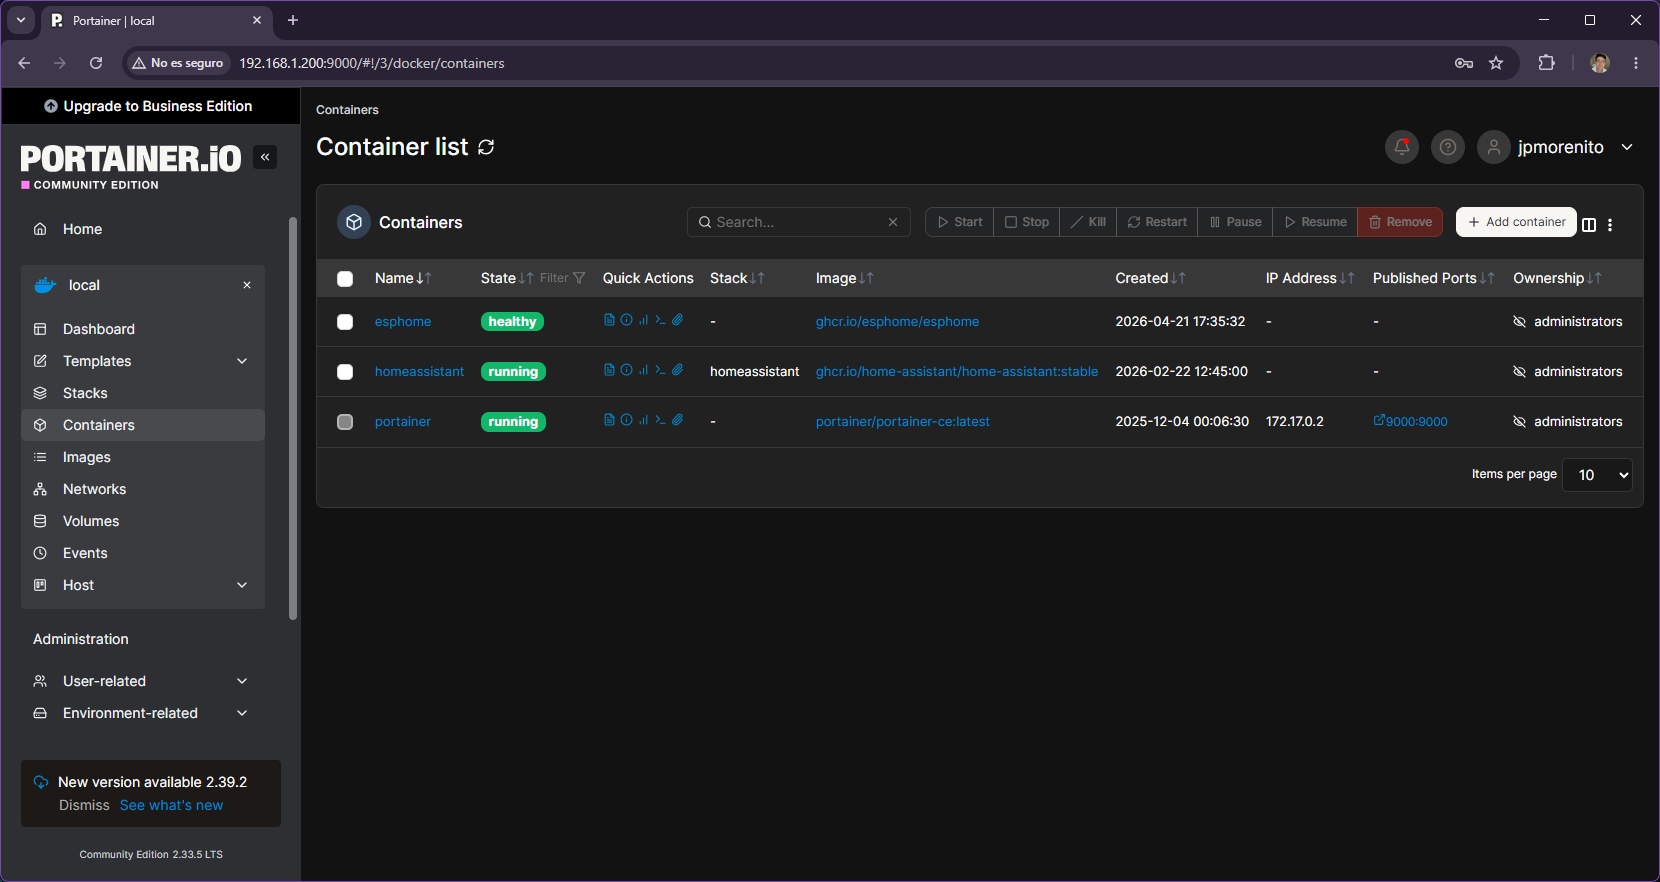
\includegraphics[width=0.95\textwidth]{Img/portainer_containers.png}
        \caption{Interfaz de administración de contenedores Docker (Portainer) corriendo en la Raspberry Pi 4.}
        \label{fig:portainer_containers}
    \end{figure}

    \item \textbf{Inyección de firmware y ubicación física:} creación y compilación de los archivos de configuración declarativos (YAML) empleando el compilador cruzado de ESPHome para generar ejecutables optimizados en C++. El \textit{firmware} se transfirió inicialmente a través de conexión física USB y posteriormente mediante actualizaciones inalámbricas OTA (\textit{Over-the-Air}). Se validó la comunicación cifrada local mediante la API nativa de ESPHome, la cual opera mediante un socket TCP persistente utilizando el protocolo Noise y serialización binaria Protocol Buffers. Tras comprobar la conexión inalámbrica local estable, los microcontroladores ESP32 y sus sensores se instalaron en sus cajas protectoras y ubicaciones definitivas.
    \item \textbf{Ejecución del plan de pruebas e integración:} aplicación de estímulos físicos controlados sobre el entorno (variación de luz, generación de sonido, cruce de barreras y aperturas de acceso) para auditar el comportamiento lógico de los actuadores y realizar el ajuste fino de los tiempos de retraso y las transiciones del motor contextual en el servidor central.
\end{enumerate}

\subsection{Configuración y ensamblaje de nodos}
\label{sec:conexionado}
El conexionado eléctrico y la asignación de pines de los módulos empotrados se diseñaron respetando estrictamente los niveles lógicos de tensión eléctrica. Se aseguró que los buses de datos digitales y las salidas de los divisores resistivos no superasen el límite de tolerancia de 3.3\,V impuesto por los pines GPIO del SoC ESP32.

\begin{itemize}
    \item \textbf{Nodo Ambiente:} el sensor de temperatura y humedad DHT11 se conecta mediante un bus digital unifilar (\textit{single-wire}) al pin GPIO 4. El fotorresistor (LDR) se integra en un circuito divisor de tensión analógico, cuya salida de voltaje se introduce directamente al pin GPIO 32 para ser digitalizada por el convertidor analógico-digital (ADC) interno del microcontrolador. El relé de estado sólido, que actúa como interruptor de potencia para controlar la luminaria principal de la habitación, se gobierna mediante una señal de salida digital en el pin GPIO 26. Por su parte, el transductor acústico (Big Sound) se conecta exclusivamente por vía digital al pin GPIO 27. El filtrado de rebotes e interrupciones repetitivas provocadas por picos de sonido cortos se realiza mediante un filtro de retardo por software en el \textit{firmware} de ESPHome (\texttt{delayed\_off: 500ms}) como se detalla en el Código~\ref{lst:esphome_sonido}, mientras que la calibración de la sensibilidad se efectúa físicamente mediante el potenciómetro analógico integrado en el módulo de sonido.

\begin{lstlisting}[language=YAML, caption={Declaración del transductor acústico y su filtro en el firmware de ESPHome (Nodo Ambiente).}, label={lst:esphome_sonido}]
binary_sensor:
  - platform: gpio
    pin: 27
    name: 'Detector de Sonido'
    device_class: sound
    filters:
      - delayed_off: 500ms # Filtro para evitar multiples rebotes
\end{lstlisting}

    \item \textbf{Nodo Escritorio:} la interfaz del radar de ondas milimétricas FMCW (HLK-LD2410) se conecta al bus serie UART del ESP32, requiriendo el cruce de los canales de comunicación: el pin de transmisión (TX) del radar se conecta al pin GPIO 16 (configurado como RX en el microcontrolador) y el pin de recepción (RX) del radar se conecta al pin GPIO 17 (TX en el microcontrolador), operando de forma asíncrona a una tasa de transferencia de 256\,000 baudios para garantizar la tasa de refresco requerida por la telemetría espacial.
    \item \textbf{Nodo Puerta:} el sensor de puerta magnético (interruptor Reed) se conecta entre el pin GPIO 4 y el plano de masa física (GND). Mediante el \textit{firmware} de ESPHome se activa la resistencia de polarización de subida (\textit{pull-up}) interna del microcontrolador, garantizando una lectura lógica alta (3.3\,V) estable cuando el contacto está abierto, la cual cae instantáneamente a un nivel lógico bajo (0\,V) cuando el imán de la hoja de la puerta cierra mecánicamente el circuito. Asimismo, el módulo de diodo emisor láser semiconductor se conecta a una salida digital en el pin GPIO 5, gobernado de forma directa por la máquina de estados de seguridad perimetral para actuar como barrera visual disuasoria en el umbral del acceso principal. Los fragmentos clave de esta configuración se listan en el Código~\ref{lst:esphome_puerta}.

\begin{lstlisting}[language=YAML, caption={Fragmentos clave del firmware del Nodo Puerta en ESPHome.}, label={lst:esphome_puerta}]
binary_sensor:
  - platform: gpio
    pin:
      number: 4
      mode:
        input: true
        pullup: true # Habilita la pull-up interna del ESP32
    name: 'Sensor Puerta'
    device_class: door
    filters:
      - delayed_on: 100ms
      - delayed_off: 100ms

switch:
  - platform: gpio
    pin: 5
    name: 'Laser Puerta'
    id: laser_puerta
    restore_mode: ALWAYS_OFF # Empieza apagado por seguridad
\end{lstlisting}
\end{itemize}

\subsection{Pruebas unitarias y de caja negra}
\label{sec:pruebas_caja_negra}
Con carácter previo a la integración en red del sistema completo, cada nodo físico se sometió a un protocolo de pruebas de caja negra para certificar la correspondencia exacta entre los estímulos del entorno y el comportamiento de los componentes:
\begin{itemize}
    \item \textbf{Diagnóstico de la instrumentación analógica:} se utilizó instrumentación de laboratorio (multímetro digital) para registrar la tensión de salida del circuito divisor de tensión del LDR frente a variaciones de flujo luminoso. Esta prueba permitió calibrar el comportamiento del ADC y descartar defectos de fabricación en las soldaduras físicas (como falsos contactos o derivaciones), previniendo la inyección de lecturas anómalas en el microcontrolador.
    \item \textbf{Calibración del rango y sensibilidad del radar:} el radar FMCW (HLK-LD2410) se evaluó monitorizando el bus serie UART mediante comandos de depuración en caliente para contrastar la sectorización espacial teórica con el comportamiento real. Se determinó que los micromovimientos provocados por elementos inanimados oscilantes (tales como corrientes de aire en las cortinas) generaban falsas detecciones de energía en rangos lejanos. Este ruido se mitigó ajustando dinámicamente, mediante la consola de configuración, los umbrales de sensibilidad en las compuertas de distancia (\textit{distance gates}) correspondientes, logrando aislar exclusivamente la presencia humana real. La interfaz de monitorización de compuertas en el servidor ESPHome se ilustra en la Figura~\ref{fig:esphome_radar_diag}.
\end{itemize}

\begin{figure}[H]
    \centering
    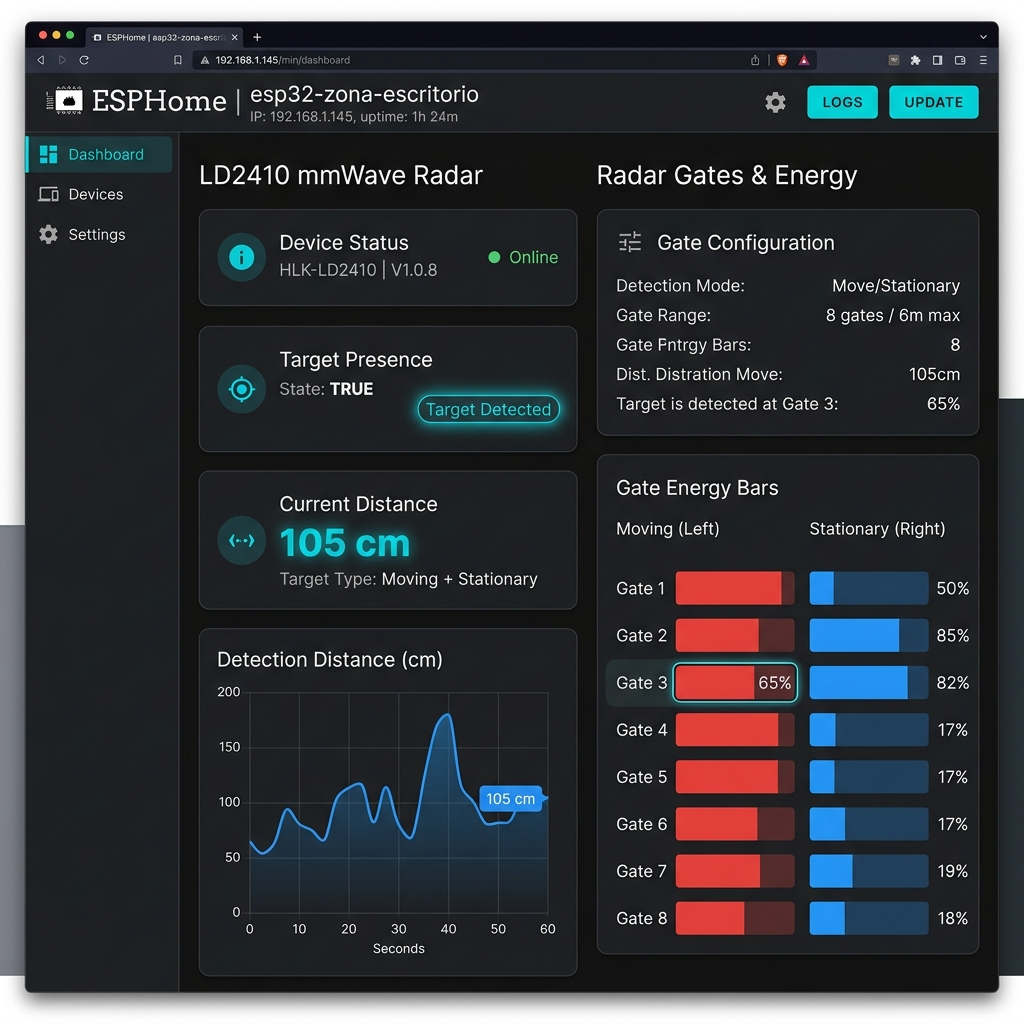
\includegraphics[width=0.95\textwidth]{Img/esphome_radar_diag.png}
    \caption{Panel de monitorización en tiempo real de compuertas y sensibilidad en ESPHome para el radar LD2410.}
    \label{fig:esphome_radar_diag}
\end{figure}

\subsection{Pruebas de integración}
\label{sec:pruebas_integracion}
Superada la fase de validación aislada de los componentes del hardware, se evaluó la cohesión global de las comunicaciones perimetrales (API nativa de ESPHome), la persistencia local y la ejecución de las automatizaciones en el servidor central:
\begin{itemize}
    \item \textbf{Evaluación de ergonomía proactiva (Pomodoro Espacial):} se simuló un estado de presencia ininterrumpida en el área de trabajo en modo de estudio. Al alcanzarse los 50 minutos de actividad continua definidos en la regla de negocio (\texttt{input\_select.estado\_habitacion} en estado \texttt{Estudio}), el servidor central procesó la telemetría e inició con éxito la acción del parpadeo intermitente de la iluminación física (mediante la conmutación secuencial del GPIO 26 en intervalos de un segundo) y envió la alerta asíncrona \textit{push} al terminal móvil del usuario a través del servicio de notificación centralizado, logrando interrumpir al usuario para evitar la fatiga cognitiva.
    \item \textbf{Evaluación de tolerancia a fallos lógicos:} para verificar la resiliencia del motor contextual bayesiano ante fallos de lectura, se simuló el bloqueo en nivel analógico bajo del fotorresistor (LDR), lo que induciría teóricamente al sistema a deducir erróneamente un estado de descanso (\texttt{Durmiendo}). A continuación, se procedió a evacuar la estancia por completo. Al no registrarse micromovimientos en el radar de ondas milimétricas en el Nodo Escritorio (\texttt{binary\_sensor.esp32\_zona\_escritorio\_ocupacion\_general} en estado apagado) y transcurrir el margen de tiempo de seguridad de la regla de inactividad, el motor de contexto bayesiano invalidó la lectura anómala del sensor lumínico y forzó la transición lógica directa al estado seguro de \texttt{Ausente}. El código YAML que rige esta transición en el servidor central se lista en el Código~\ref{lst:ha_inactividad}, y el panel general Lovelace con las métricas activas se ilustra en la Figura~\ref{fig:ha_lovelace_dashboard}.
    
\begin{lstlisting}[language=YAML, caption={Automatización de ausencia automática por inactividad en Home Assistant (automations.yaml).}, label={lst:ha_inactividad}]
- id: '1779447855314'
  alias: 'Contexto: Ausencia Automatica por Inactividad'
  description: Pasa la habitacion a Ausente tras detectar inactividad prolongada
  trigger:
    - entity_id: binary_sensor.esp32_zona_escritorio_ocupacion_general
      to: 'off'
      for: 00:00:10 # Reducido a 10s en el laboratorio para pruebas rapidas
      trigger: state
  condition:
    - condition: not
      conditions:
        - condition: state
          entity_id: input_select.estado_habitacion
          state: Ausente
  action:
    - target:
        entity_id: input_select.estado_habitacion
      data:
        option: Ausente
      action: input_select.select_option
  mode: single
\end{lstlisting}

    \begin{figure}[H]
        \centering
        \begin{subfigure}[b]{0.85\textwidth}
            \centering
            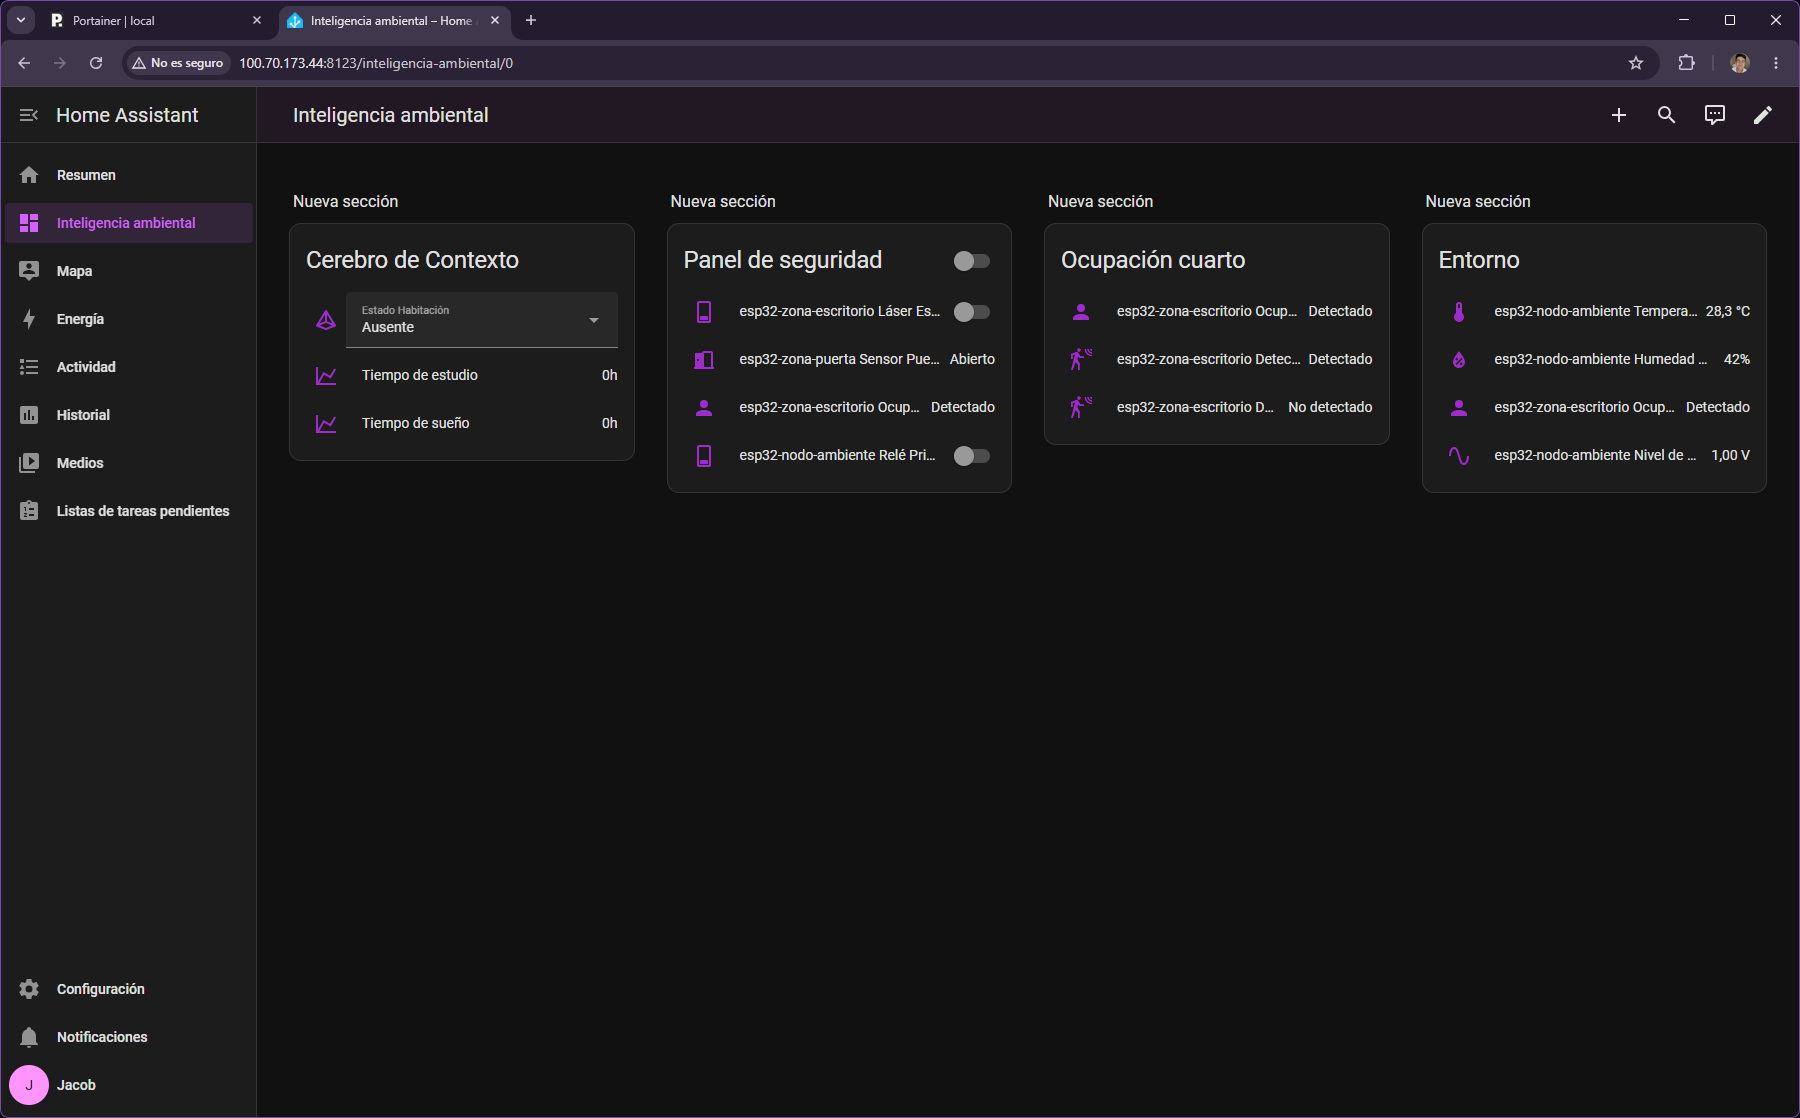
\includegraphics[width=\textwidth]{Img/ha_dashboard_lovelace1.png}
            \caption{Vista general de tarjetas y sensores.}
            \label{fig:ha_lovelace_1}
        \end{subfigure}
        
        \vspace{6mm}
        \begin{subfigure}[b]{0.85\textwidth}
            \centering
            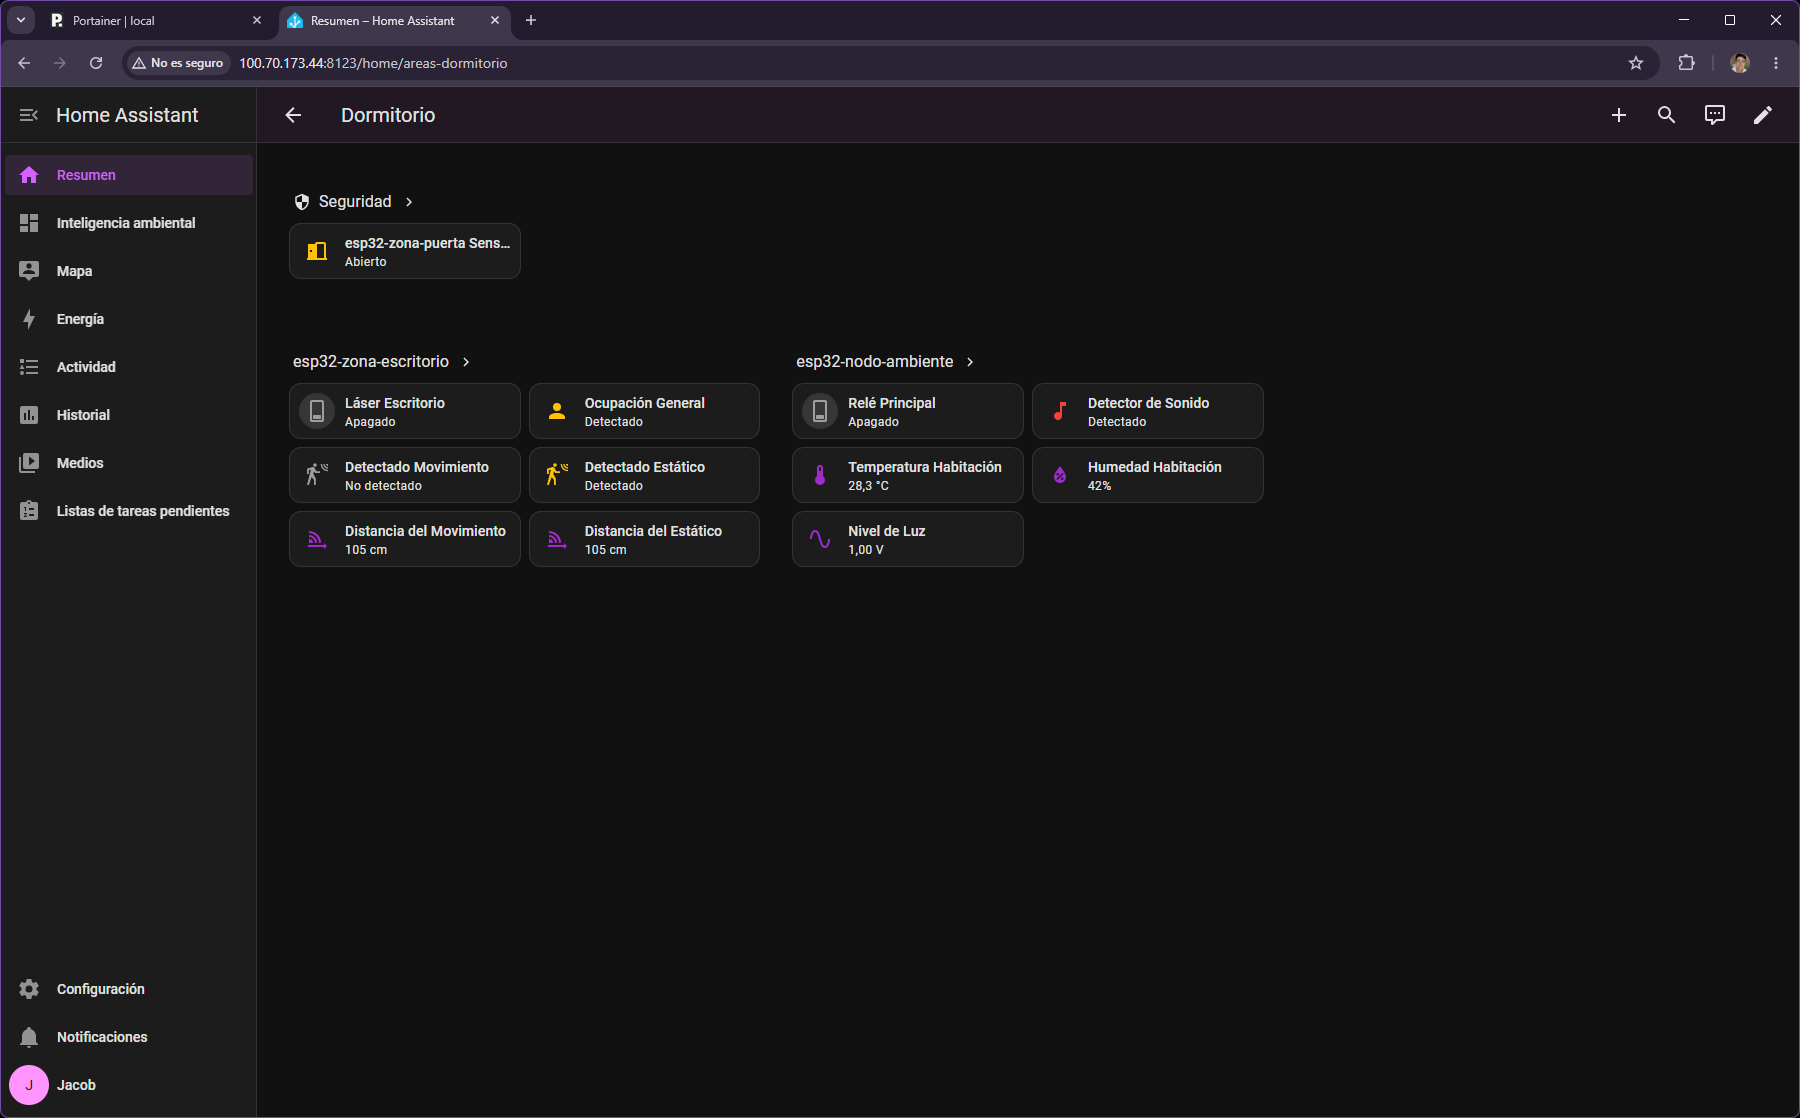
\includegraphics[width=\textwidth]{Img/ha_dashboard_lovelace2.png}
            \caption{Historial de estados y estadísticas.}
            \label{fig:ha_lovelace_2}
        \end{subfigure}
        \caption{Cuadros de mando Lovelace en Home Assistant mostrando las telemetrías y transiciones contextuales.}
        \label{fig:ha_lovelace_dashboard}
    \end{figure}

    \par\vspace{3mm}
    \colorbox{gray!10}{%
    \begin{minipage}{0.95\textwidth}
    \textbf{Nota sobre los parámetros temporales de prueba:} Con el propósito de verificar esta automatización de inactividad de forma ágil durante los ensayos en el laboratorio de pruebas y la posterior demostración ante el tribunal de evaluación académica, el retardo temporal de ausencia se redujo temporalmente en el archivo de automatizaciones de Home Assistant (\texttt{automations.yaml}) de los 20 minutos teóricos de producción a un valor de prueba de 10 segundos (\texttt{for: 00:00:10}), restaurando la lógica al retardo completo tras verificar su resiliencia.
    \end{minipage}%
    }
\end{itemize}

\subsection{Resultados experimentales en entorno real}
\label{sec:resultados_experimentales}
Los ensayos empíricos realizados en un entorno real de uso demuestran que la arquitectura domótica local responde con solidez a los requisitos operacionales. La redundancia y fusión de sensores aplicada al motor bayesiano elimina por completo los falsos negativos de presencia inherentes a la sensórica pasiva infrarroja (PIR) tradicional, logrando que el estado contextual del entorno se mantenga estable e inalterado en presencia de actividades estáticas como el estudio, la lectura o el descanso.

Asimismo, las mediciones de latencia en la red local inalámbrica evidencian que el tiempo transcurrido desde que se produce un cambio físico en un pin (como la separación mecánica del interruptor magnético de la puerta) hasta su persistencia y registro en la base de datos de Home Assistant se sitúa de forma sostenida por debajo del umbral de 150\,ms. Este valor valida la idoneidad del paradigma de computación perimetral (\textit{Edge Computing}) y la sustitución de servidores remotos en la nube o agentes con intermediarios complejos de comunicación, proporcionando un entorno seguro, de respuesta instantánea y respetuoso con la privacidad de los datos locales del usuario.
